\documentclass{article}

\usepackage{subcaption}
\usepackage{graphicx}
\usepackage{amsmath}
\usepackage{color}
\usepackage{fullpage}
\usepackage{pgfgantt}
\usepackage{booktabs}
\usepackage{tabularx}
\usepackage{relsize}
\usepackage{epigraph}
\usepackage{parskip}
\usepackage{float}
\usepackage{listings}
\usepackage{tcolorbox}
\usepackage{program}
\usepackage{pgfplots}

\renewcommand{\familydefault}{\sfdefault}

\definecolor{pr0}{RGB}{61, 255, 12}
\definecolor{pr1}{RGB}{208, 231, 11}
\definecolor{pr2}{RGB}{255, 190, 0}
\definecolor{pr3}{RGB}{231, 149, 11}
\definecolor{pr4}{RGB}{255, 95, 6}
\definecolor{pr5}{RGB}{231, 20, 3}
\definecolor{pr6}{RGB}{255, 12, 190}

\definecolor{codeblue}{HTML}{528bff}
\definecolor{codegreen}{HTML}{98C379}
\definecolor{codepurple}{HTML}{C678DD}
\definecolor{codebg}{gray}{0.92}

\newtcbox{\codeinline}{nobeforeafter,colframe=codebg,colback=codebg,arc=1pt,boxrule=0.5pt, left=0.5pt,right=0.5pt,top=0.5pt,bottom=0.5pt,tcbox raise base}

\newcommand{\code}[1]{\codeinline{\texttt{#1}}}

\lstdefinestyle{cpp}{
  language=C++,
  basicstyle=\ttfamily,
  backgroundcolor=\color{codebg},
  numberstyle=\color{black},
  keywordstyle=\color{codeblue},
  commentstyle=\color{codegreen},
  stringstyle=\color{codepurple},
  breakatwhitespace=false,
  breaklines=true,
  columns=flexible,
  keepspaces=true,
  firstnumber=1,
  numbers=left,
  numbersep=3pt,
  tabsize=4,
  title=\lstname
}

\lstset{escapechar=@,style=cpp}

\title{Optimal Sorting Algorithms\\Visualization and Comparison}
\date{\today}
\author{Martin Nestorov}
\linespread{1}

\begin{document}

\maketitle
\pagenumbering{arabic}

\newpage

\section{\underline{Introduction}}

There are several sorting algorithms that are quite popular and have a wide range of uses in real world applications. In general, they employ a different approach to solving the problem of sorting a set of numbers. Because we are dealing with sorting algorithms, we are developing solutions based on comparison between values, picking the largest or smallest of the two.

The chosen algorithms for this topic are as follows:

\begin{itemize}
\item \textbf{Merge Sort}
\item \textbf{Quick Sort}
\item \textbf{Binary Tree Sort}
\item \textbf{Heap Sort}
\item \textbf{Shell Sort}
\end{itemize}

Each of these algorithms will be explained how it works and how it was implemented.

\subsection{\underline{Merge Sort}}

Merge sort is an efficient comparison sorting algorithm, based on the \textit{divide-and-conquer} technique. It's considered to be a stable sort, which means that the order of equal elements is the same in the input and output.

In general, the algorithm works as follow:
\begin{itemize}
\item Divide the unsorted list into $n$ sub-lists, each containing one element, where a list of one element is considered sorted.
\item Repeatedly merge sublists to produce new sorted sub-lists until there is only one sublist remaining. This will be the sorted list.
\end{itemize}

Let's look at the code of the algorithm.

We have a merging step. We separate the array into two parts and then we merge them together based on which number is bigger in the two arrays.

\begin{lstlisting}
void merge(array, left, middle, right)
{
	i, j, k;
	n1 = middle - left + 1;
	n2 = right - middle;

	<vector> L(n1), R(n2);

	for (i = 0; i < n1; i++)
	    L[i] = array[left + i];

	for (j = 0; j < n2; j++)
	    R[j] = array[middle + 1 + j];

	i = 0;
	j = 0;
	k = left;

	while (i < n1 && j < n2) {
	    if (L[i].h <= R[j].h) {
		array[k] = L[i];
		i++;
	    } else {
		array[k] = R[j];
		j++;
	    }
	    k++;
	}

	while (i < n1) {
	    array[k] = L[i];
	    i++;
	    k++;
	}

	while (j < n2) {
	    array[k] = R[j];
	    j++;
	    k++;
	}
}
\end{lstlisting}

and we call the sorting algorithm like so. First we divide it \textit{recursively} and then we merge all of the pieces on by one.

\begin{lstlisting}
void merge_sort(array, left, right)
{
    if (left < right) {
        int middle = left + (right - left) / 2;

        merge_sort(array, left, middle);
	    merge_sort(array, middle + 1, right);

        merge(array, left, middle, right);
    }
}
\end{lstlisting}

In sorting $n$ objects, merge sort has an \textbf{average} and \textbf{worst-case} performance of $O(n\ log\ n)$. If the running time of merge sort for a list of length $n$ is $T(n)$, then the recurrence $T(n) = 2T(n/2) + n$ follows from the definition of the algorithm (apply the algorithm to two lists of half the size of the original list, and add the $n$ steps taken to merge the resulting two lists).

Merge sort's most common implementation does not sort in place. The memory size of the input must be allocated for the sorted output to be stored in.

We can visualize this algorithm through a diagram like so

\begin{figure}[H]
  \centering
  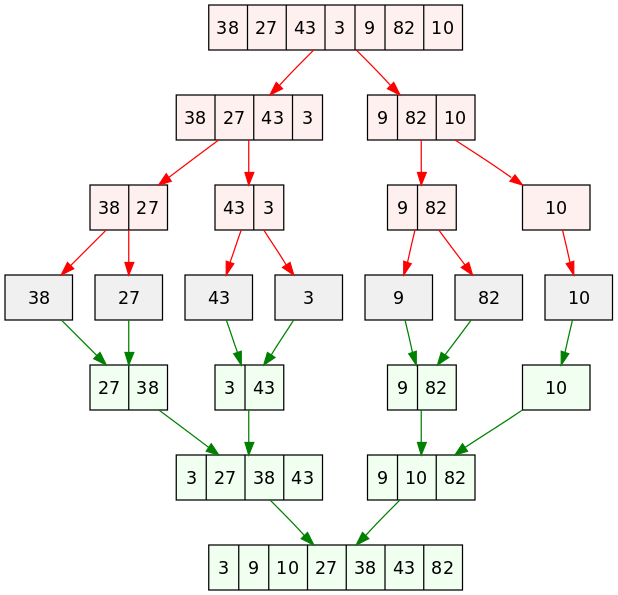
\includegraphics[scale=0.4]{./Merge_sort_algorithm_diagram.png}
  \caption{Merge Sort}
  \label{fig:Merge Sort}
\end{figure}

In summary, the merge sort algorithm has these complexities

\begin{table}[H]
  \begin{center}
    \label{tab:Merge Sort Complexity}
    \begin{tabular}{c|c}
      \toprule
      \textbf{Case} & \textbf{Time Complexity} \\
      \midrule
      Worst Case & $O(n\ log\ n)$ \\
      Average Case & $O(n\ log\ n)$ or $O(n)$ \\
      Best Case & $O(n\ log\ n)$ \\
      \bottomrule
      \toprule
      \textbf{Case} & \textbf{Space Complexity} \\
      \midrule
      Worst Case & $O(n)$ \\
    \end{tabular}
    \caption{Merge Sort Complexity}
  \end{center}
\end{table}

\subsection{\underline{Quick Sort}}

Quicksort is an $O(n\ log\ n)$ efficient sorting algorithm. In efficient implementations it is not a stable sort, meaning that the relative order of equal sort items is not preserved. Quicksort can operate in-place on an array, requiring small additional amounts of memory to perform the sorting. It is very similar to selection sort, except that it does not always choose worst-case partition.

Quicksort, on average, takes $O(n\ log\ n)$ comparisons to sort $n$ items. In the worst case, it makes $O(n2)$ comparisons, though this behavior is rare.

Quicksort is a divide-and-conquer algorithm. Quicksort first divides a large array into two smaller sub-arrays: the low elements and the high elements. Quicksort can then recursively sort the sub-arrays. The steps are:
\begin{itemize}
\item Pick an element, called a pivot, from the array.
\item Partitioning: reorder the array so that all elements with values less than the pivot come before the pivot, while all elements with values greater than the pivot come after it (equal values can go either way). After this partitioning, the pivot is in its final position.
\item Recursively apply the above steps to the sub-array of elements with smaller values and separately to the sub-array of elements with greater values.
\end{itemize}

The pivot selection and partitioning steps can be done in several different ways; the choice of specific implementation schemes greatly affects the algorithm's performance. In this case the pivot is chosen to be the high value of the array.

\begin{lstlisting}
void quick_sort(array, low, high)
{
	if (high > low)
	{
	    pivot = partition(array, low, high);
	    quick_sort(array, low, pivot - 1);
	    quick_sort(array, pivot + 1, high);
	}
}
\end{lstlisting}

The partitioning of the algorithm would look like so:

\begin{lstlisting}
int partition(array, low, high)
{
	pivot = array[high];
	i = low - 1;

	for (j = low; j <= high - 1; j++) {
	    if (array[j] <= pivot) {
		i++;
		swap(array[i], array[j]);
	    }
	}

	swap(array[i + 1], array[high]);

	return i + 1;
}
\end{lstlisting}

We can also see a diagram that shows how the quick sort will work.

\begin{figure}[H]
  \centering
  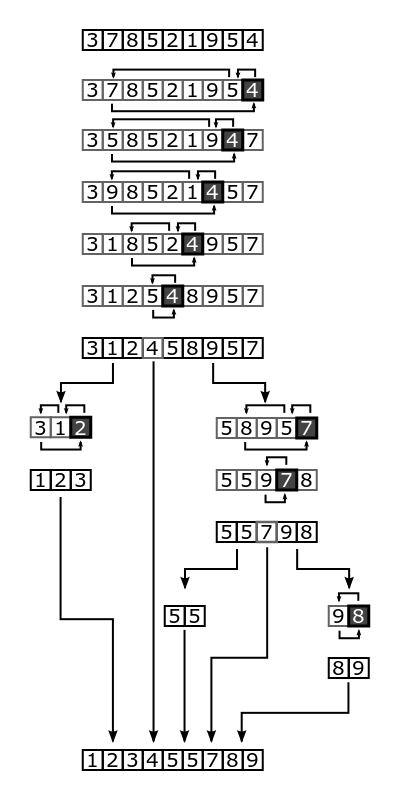
\includegraphics[scale=0.4]{./Quicksort-diagram.png}
  \caption{Quick Sort}
  \label{fig:Quick Sort}
\end{figure}

In summary, the quick sort algorithm has these complexities

\begin{table}[H]
  \begin{center}
    \label{tab:Quick Sort Complexity}
    \begin{tabular}{c|c}
      \toprule
      \textbf{Case} & \textbf{Time Complexity} \\
      \midrule
      Worst Case & $O(n^2)$ \\
      Average Case & $O(n\ log\ n)$ \\
      Best Case & $O(n\ log\ n)$ \\
      \bottomrule
      \toprule
      \textbf{Case} & \textbf{Space Complexity} \\
      \midrule
      Worst Case & $O(n)$ \\
    \end{tabular}
    \caption{Quick Sort Complexity}
  \end{center}
\end{table}

\subsection{\underline{Binary Tree Sort}}

A tree sort is a sort algorithm that builds a binary search tree from the elements to be sorted, and then traverses the tree (in-order) so that the elements come out in sorted order.

Adding one item to a binary search tree is on average an $O(log\ n)$ process. Adding $n$ items is an $O(n\ log\ n)$ process, making tree sorting a 'fast sort' process. Adding an item to an unbalanced binary tree requires $O(n)$ time in the worst-case.

The worst-case behavior can be improved by using a self-balancing binary search tree. Using such a tree, the algorithm has an $O(n\ log\ n)$ worst-case performance, thus being optimal for a comparison sort. However, trees require memory to be allocated on the heap, which is a significant performance hit when compared to quicksort and heapsort.

The implementation of the balancing tree is big, but the insertion part is what is interesting to us, so we can see its implementation.

\begin{lstlisting}
void insert(node root, key)
{
    if (root == nullptr) {
        root = new node(key, nullptr, nullptr);
    } else if (key <= root->key) {
        insert(root->left, key);

        if (height(root->left) - height(root->right) == 2) {
            if (key <= root->left->key)
                left_rotation(root);
            else
                double_left_rotation(root);
        }
    } else if (key > root->key) {
        insert(root->right, key);

        if (height(root->right) - height(root->left) == 2) {
            if (key > root->right->key )
                right_rotation(root);
            else
                double_right_rotation(root);
        }
    }

    root->height = max(height(root->left), height(root->right)) + 1;
}
\end{lstlisting}

We can see that we are re-balancing the tree with the left and right rotations upon insertion, when the height of the tree grows too big.

And then in order to sort the elements, we can do an in-order traversal.

\begin{lstlisting}
void in_order_traversal(node root)
{
    if (root != nullptr) {
        in_order_traversal(root->left);

        print(key);

	in_order_traversal(root->right);
    }
}
\end{lstlisting}

In a diagram, the logic flow would look like this:

\begin{figure}[H]
  \centering
  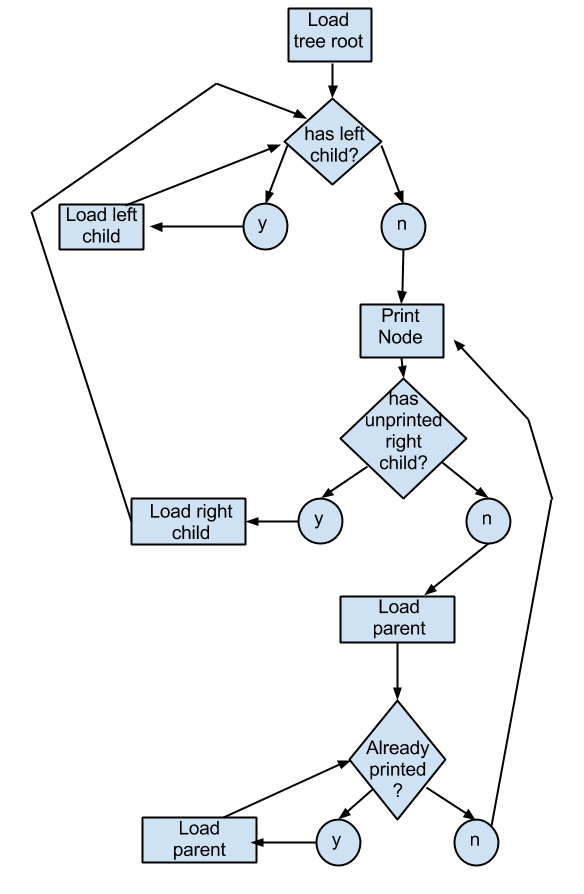
\includegraphics[scale=0.4]{./binary_tree.png}
  \caption{Binary Tree Sort}
  \label{fig:Binary Tree Sort}
\end{figure}

In summary, the binary tree sort algorithm has these complexities

\begin{table}[H]
  \begin{center}
    \label{Binary Tree Sort Complexity}
    \begin{tabular}{c|c}
      \toprule
      \textbf{Case} & \textbf{Time Complexity} \\
      \midrule
      Worst Case & $O(n\ log\ n)$ \\
      Average Case & $O(n\ log\ n)$ \\
      Best Case & $O(n\ log\ n)$ \\
      \bottomrule
      \toprule
      \textbf{Case} & \textbf{Space Complexity} \\
      \midrule
      Worst Case & $O(n)$ \\
    \end{tabular}
    \caption{Binary Tree Sort Complexity}
  \end{center}
\end{table}

\subsection{\underline{Heap Sort}}

\textbf{Heapsort} is another optimal sorting algorithm. It divides its input into a sorted and an unsorted region, and it iterativelly shrinks the unsorted region by extracting the largest element and moving that to the sorted region. Like the name suggests, it uses a heap data structure rather than a linear-time search to find the maximum number. In this case, we are using the so called max-heap tree, where the maximum number sits at the root of the tree.

It has a worst-case $O(n\ log\ n)$ run-time. \textbf{Heapsort} is an in-place algorithm, but it is not a stable sort.

\textbf{Heapsort} can be divided into two parts. In the first step, a \textit{heap} is built out of the data. The heap is often placed in an array with the layout of a complete binary tree. The complete binary tree maps the binary tree structure into the array indices, where each array index represents a node in the tree.

In the second step, a sorted array is created by repeatedly removing the largest element from the heap (the root of the heap), and inserting it into the array. The heap is updated after each removal to maintain the heap property. Once all objects have been removed from the heap, the result is a sorted array.

The heapsort algorithm involves preparing the list by first turning it into a max heap. The algorithm then repeatedly swaps the first value of the list with the last value, decreasing the range of values considered in the heap operation by one, and sifting the new first value into its position in the heap.

We start the implementation with an initial heapify operation on the array, and then we sequentially swap the values until we are done.

\begin{lstlisting}
void heap_sort(array)
{
	for (i = array.size() / 2 - 1; i >= 0; i--)
	    heapify(array, array.size(), i);

	for (i = array.size() - 1; i >= 0; i--) {
	    swap(array[0], array[i]);
	    heapify(array, i, 0);
	}
}
\end{lstlisting}

The heap step is then implemented like this:

\begin{lstlisting}
void heapify(array, n, i)
{
	largest = i;
	l = 2 * i + 1;
	r = 2 * i + 2;

	if (l < n && array[l] > array[largest])
	    largest = l;

	if (r < n && array[r] > array[largest])
	    largest = r;

	if (largest != i) {
	    swap(array[i], array[largest]);
	    heapify(array, n, largest);
	}
}
\end{lstlisting}

In summary, the heap sort algorithm has these complexities

\begin{table}[H]
  \begin{center}
    \label{tab:Heap Sort Complexity}
    \begin{tabular}{c|c}
      \toprule
      \textbf{Case} & \textbf{Time Complexity} \\
      \midrule
      Worst Case & $O(n\ log\ n)$ \\
      Average Case & $O(n\ log\ n)$ \\
      Best Case & $O(n\ log\ n)$ or $O(n)$ \\
      \bottomrule
      \toprule
      \textbf{Case} & \textbf{Space Complexity} \\
      \midrule
      Worst Case & $O(n)$ \\
    \end{tabular}
    \caption{Heap Sort Complexity}
  \end{center}
\end{table}

\subsection{\underline{Shell Sort}}

Shellsort is an in-place comparison sort. It can be seen as sorting by insertion (insertion sort). The method starts by sorting pairs of elements far apart from each other, then progressively reducing the gap between elements to be compared. Starting with far apart elements, it can move some out-of-place elements into position faster than a simple nearest neighbor exchange. The running time of Shellsort is heavily dependent on the gap sequence it uses.

The idea is to arrange the list of elements so that, starting anywhere, considering every $h-th$ element gives a sorted list. Such a list is said to be $h$-sorted. Beginning with large values of $h$, this rearrangement allows elements to move long distances in the original list, reducing large amounts of disorder quickly, and leaving less work for smaller $h$-sort steps to do. If the list is then $k$-sorted for some smaller integer $k$, then the list remains $h$-sorted. Following this idea for a decreasing sequence of $h$ values ending in 1 is guaranteed to leave a sorted list in the end.

\begin{lstlisting}
void shell_sort(array)
{
	for (gap = array.size() / 2; gap > 0; gap /= 2)
	{
	    for (i = gap; i < array.size(); i += 1)
	    {
		temp = array[i];
		j;
		for (j = i; j >= gap && array[j - gap] > temp; j -= gap)
		    array[j] = array[j - gap];

		array[j] = temp;
	    }
	}
}
\end{lstlisting}

The question of deciding which gap sequence to use is difficult. Every gap sequence that contains 1 yields a correct sort (as this makes the final pass an ordinary insertion sort); however, the properties of thus obtained versions of Shellsort may be very different. Too few gaps slows down the passes, and too many gaps produces an overhead.

In this case, we start off with a gap that is half the size of the initial array, and then we shrink it by two-fold each iteration.

In summary, the shell sort algorithm has these complexities

\begin{table}[H]
  \begin{center}
    \label{tab:Shell Sort Complexity}
    \begin{tabular}{c|c}
      \toprule
      \textbf{Case} & \textbf{Time Complexity} \\
      \midrule
      Worst Case & $O(n^2)$ or $O(n\ log\ n)$ \\
      Average Case & depends on gap sequence \\
      Best Case & $O(n\ log\ n)$ \\
      \bottomrule
      \toprule
      \textbf{Case} & \textbf{Space Complexity} \\
      \midrule
      Worst Case & $O(n)$ \\
    \end{tabular}
    \caption{Shell Sort Complexity}
  \end{center}
\end{table}

\section{\underline{Testing}}

In order to test these algorithms, a random number generator is created so that a good set would be evaluated each time. Thus the number generator generates several types of sets, each one showing how the different algorithms sort the set.

The testing is done on 3 different types of number sets. One is the random set, which is generated with a uniform distribution. Another one is done on a sequential number set, which has been shuffled randomly. The last is a set which is sequential, but put in reverse order.

By having these 3 types of sets, we can see how the algorithms are handling repeating values, and how the perform on completely reversed sets.

\subsection{\underline{Random Number Generation}}

The generator is implemented using the standard \code{C++} library, using the \code{<random>} header file.

When generating numbers for the purpose of sorting them, we want them to be as even as possible. Thus, an uniform distribution across all numbers is vital. The number generator is implemented like so:

\begin{lstlisting}
std::mt19937 rng {std::random_device()()};
std::uniform_int_distribution<int> even_rand(0, max);
even_rand(rng);
\end{lstlisting}

We have a Marsenne Twister number generator, which is seeded by a random device, which would be some part of the hardware. Then we have a uniform distribution, which is in the range of 0 to some number max. Then, when we generate a number each time, we call the \code{even\_rand(rng)} statement. Because of this, we guarantee, that there is no bias in our data set.

If we want to have a sequence of numbers, but to put them in a randomized order, we can do the following.

\begin{lstlisting}
std::random_shuffle(num_set.begin(), num_set.end());
\end{lstlisting}

This would take the set and randomize it without any bias in it. Visually, this would look very similar to the random set, but it will not contain any duplicate numbers.

\section{\underline{Visualization}}

Visualization of this project is done through the \code{SDL2} graphics library, where each number is represented by a rectangle, and the height is the number we are sorting.

\begin{lstlisting}
SDL_Rect rect = {x, y, width, height (value_to_sort)};
\end{lstlisting}

We populate the screen with these rectangles and then we sort them with each algorithm.

\section{\underline{Timing}}

Each algorithm is timed for how long it runs in milliseconds. As it is expected, when we are visualizing the algorithms, the time for large sets of numbers increases. When we are not doing any visualization, the time for completion shrinks exponentially.

Here is a summary of the different times for the different algorithms with all of the results being in milliseconds.

\begin{table}[H]
  \begin{center}
    \label{tab:FCFS times}
    \begin{tabular}{c|c|c|c|c}
      \toprule
      \textbf{Number Set} & \textbf{Merge Sort} & \textbf{Quick Sort} & \textbf{Heap Sort} & \textbf{Shell Sort} \\
      \midrule
      1 mil & 622.2 & 299.3 & 579.1 & 791.7 \\
      500 k & 299.4 & 139.9 & 270.0 & 351.5 \\
      10 k & 5 & 2 & 4 & 3.6 \\
      \bottomrule
      \toprule
      \textbf{Visualization} \\
      1280 & 20633 & 27248 & 20595 & 19436 \\
    \end{tabular}
    \caption{Average running times}
  \end{center}
\end{table}

What is interesting to us is the fact that the Quick sort and the Heap sort are the fastest from all, regardless of the fact that Quick sort is considered to be an unstable sorting algorithm.

All of these values are the average from 10 experiments, run with the mentioned number sets.
\\
\\
\\
\textbf{Sources}

The sources used for the pictures come from various internet articles on sorting algorithms.

The information comes from testing the application as well as from the book "Introduction to Algorithms (3rd ed.)" and various internet articles.

\end{document}